\documentclass[tikz, border=10pt]{standalone}

% Required packages
\usepackage{tikz}
\usepackage{xcolor}
\usepackage{lmodern} % Use a modern, scalable font

% TikZ libraries for advanced shapes, positioning, arrows, and shadings
\usetikzlibrary{shapes.geometric, positioning, arrows.meta, shadings}

% Set the default font family to sans-serif to match the image
\renewcommand{\familydefault}{\sfdefault}

% --- Color Definitions ---
% Define custom colors sampled from the image for accuracy
\definecolor{BGColor}{HTML}{F0F2F7}      % Light grey-blue background
\definecolor{BorderColor}{HTML}{2D3748}  % Dark blue-grey for borders
\definecolor{myPurple}{HTML}{8A5CFE}     % Vibrant purple for gradients
\definecolor{myLightBlue}{HTML}{A5D8FF}  % Light blue for the 'Conv' gradient
\definecolor{myRed}{HTML}{EF4444}        % Bright red for the 'Add' gradient

% --- Shading Definitions ---
% Define the horizontal gradients (shadings) used in the blocks
\pgfdeclarehorizontalshading{conv_shading}{100bp}
{color(0bp)=(myPurple); color(100bp)=(myLightBlue)}

\pgfdeclarehorizontalshading{add_shading}{100bp}
{color(0bp)=(myPurple); color(100bp)=(myRed)}

\begin{document}

% Set the page background color to match the image
\pagecolor{BGColor}

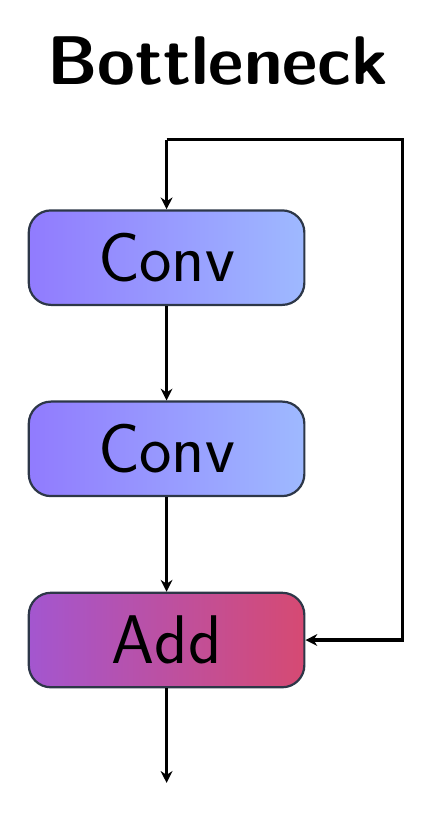
\begin{tikzpicture}[
    % Set a standard node distance for positioning
    node distance=1.2cm and 1cm
]
    % --- Style Definitions ---
    % Style for the main blocks (Conv, Add)
    \tikzset{
    >={Stealth[length=1.5mm, width=1.5mm]},
        block/.style={
            draw=BorderColor,           % Border color
            rounded corners=8pt,        % Rounded corners
            thick,                      % Border thickness
            text=black,                 % Text color
            minimum width=3.5cm,        % Minimum width of the block
            minimum height=1.2cm,       % Minimum height of the block
            font=\Huge\sffamily,        % Font size and family
            align=center                % Center text inside the block
        },
        % Style for the arrows connecting the blocks
        arrow/.style={
            draw=black,                 % Arrow color
            % -{{Stealth[length=4mm, width=3mm]}}, % Arrow tip style and size
            very thick            % Arrow line thickness
        }
    }

    % --- Nodes ---
    % Title node
    \node[font=\Huge\bfseries\sffamily] (title) at (0.65, 5.5) {Bottleneck};

    % We use a scope to apply styles to a group of nodes, but it's not strictly necessary here.
    % The nodes are placed relative to each other using the 'positioning' library.
    \node[block, shading=conv_shading] (conv1) at (0, 3) {Conv};
    \node[block, shading=conv_shading, below=of conv1] (conv2) {Conv};
    \node[block, shading=add_shading, below=of conv2] (add) {Add};

    % --- Connections (Arrows) ---
    % Define a coordinate for the main input point for clarity
    \coordinate (input) at (0, 4.5);

    % Main vertical data flow
    \draw[->, arrow] (input) -- (conv1.north);
    \draw[->, arrow] (conv1.south) -- (conv2.north);
    \draw[->, arrow] (conv2.south) -- (add.north);
    \draw[->, arrow] (add.south) -- ++(0, -1.2); % Arrow pointing down from the last block

    % Skip connection (residual connection)
    % This path starts at the input, goes right, then down, then left into the 'Add' block.
    % The `|-` path construction is used for clean right-angle turns.
    % It draws a horizontal line from the start point, then a vertical line to the target's y-level,
    % and finally a horizontal line to the target anchor.
    \draw[->, arrow] (input) -- ++(3,0) |- (add.east);

\end{tikzpicture}

\end{document}